\documentclass[
	paper=A4,
	twoside=false,
	parskip=full,
	chapterprefix=true,  
	appendixprefix=true,
	12pt,
	headings=normal,
	bibliography=totoc,
	titlepage=on,
	draft=false,
]{scrreprt}
\usepackage{setspace}
\usepackage{booktabs}
\usepackage{tabularx}
\usepackage[utf8]{inputenc}
\usepackage[T1]{fontenc}
\usepackage[french]{babel}
\usepackage[
	sansserif=false,
	colorize=full,
	hangsection,
	hangsubsection, 
	hangfigurecaption=false,
	colorize=full,
	colortheme=bluemagenta,
	bibsys=bibtex,
	bibfile=main,
	bibstyle=numeric,
]{cleanthesis} 
   
\usepackage{pdfpages}
\usepackage{hyperref}
\usepackage{tikz} 
\usepackage{amsmath}
\usepackage{amsfonts}
\usepackage{amssymb}
\usepackage{amsthm}
\usepackage{amsbsy}
\usepackage{biblatex}
\usepackage{makeidx}
\usepackage{framed}
\usepackage{float}
\usepackage[acronym]{glossaries}
\usepackage{listings}
\usepackage{booktabs}
\usepackage[toc,page]{appendix}
\usepackage[mode=buildnew]{standalone}
\usepackage{xparse}
\usepackage[printonlyused,withpage]{acronym}
\usepackage{graphicx}

\usepackage{xcolor}
\usepackage{listings}

\definecolor{mGreen}{rgb}{0,0.6,0}
\definecolor{mGray}{rgb}{0.5,0.5,0.5}
\definecolor{mPurple}{rgb}{0.58,0,0.82}
\definecolor{backgroundColour}{rgb}{0.95,0.95,0.92}

\lstdefinestyle{CStyle}{
    backgroundcolor=\color{backgroundColour},   
    commentstyle=\color{mGreen},
    keywordstyle=\color{magenta},
    numberstyle=\tiny\color{mGray},
    stringstyle=\color{mPurple},
    basicstyle=\footnotesize,
    breakatwhitespace=false,         
    breaklines=true,                 
    captionpos=b,                    
    keepspaces=true,                 
    numbers=left,                    
    numbersep=5pt,                  
    showspaces=false,                
    showstringspaces=false,
    showtabs=false,                  
    tabsize=2,
    language=C
}

% titelseite info
\newcommand{\Cs}{C\#}
\newcommand*{\quelle}{% 
  \footnotesize Quelle: 
} 
\graphicspath{ {img/} }
\newcommand{\norm}[1]{\left\lVert#1\right\rVert}
\newcommand{\Autor}{}
\newcommand{\MatrikelNummer}{32}
\newcommand{\Kursbezeichnung}{L3 S6 Printemps}
\newcommand{\Was}{Rendu de projet}
\newcommand{\Titel}{Rendu de projet}
\newcommand{\AbgabeDatum}{06 mai 2022}

\includeonly{
 %erklaerung
 ,introduction
 ,preparation
 ,oeuvre
 ,analyse
 ,meilleure
 ,conclusion
 %,kapitel1
 %,kapitel2
 %,einleitung
 %,technologien
 %,umsetzung
 %,deployment
}

% JavaScript

\definecolor{lightgray}{rgb}{.9,.9,.9}
\definecolor{darkgray}{rgb}{.4,.4,.4}
\definecolor{purple}{rgb}{0.65, 0.12, 0.82}

\lstdefinelanguage{JavaScript}{
  morekeywords=[1]{break, continue, delete, else, for, function, if, in,
    new, return, this, typeof, var, void, while, with},
  % Literals, primitive types, and reference types.
  morekeywords=[2]{false, null, true, boolean, number, undefined,
    Array, Boolean, Date, Math, Number, String, Object},
  % Built-ins.
  morekeywords=[3]{eval, parseInt, parseFloat, escape, unescape},
  sensitive,
  morecomment=[s]{/*}{*/},
  morecomment=[l]//,
  morecomment=[s]{/**}{*/}, % JavaDoc style comments
  morestring=[b]',
  morestring=[b]"
}[keywords, comments, strings]

\lstdefinelanguage{JSON}{
    string=[s]{"}{"},
    stringstyle=\color{blue},
    comment=[l]{:},
    commentstyle=\color{black},
}

% For inputting other files
\newcommand\inputfile[1]{%
    \InputIfFileExists{#1}{}{\typeout{No file #1.}}%
}
 
% Nicht zitierte Quellen, die trotzdem in der Bibliographie auftauchen sollen
\nocite{*}

%lsiting optionen
\lstset{language=[Sharp]C,numbers=left,numberstyle=\tiny,breaklines,tabsize=4}
 
\lstset{literate=
  {Ö}{{\"O}}1
  {Ä}{{\"A}}1
  {Ü}{{\"U}}1
  {ß}{{\ss}}1
  {ü}{{\"u}}1
  {ä}{{\"a}}1
  {ö}{{\"o}}1
}

% --------------
%  Front Matter
% --------------

\pagenumbering{roman}
\pagestyle{empty}

\begin{document}

%%%%%%%%%%%%%%%%%%%%%%%Titelseite%%%%%%%%%%%%%%%%%%%%%%%%%%%%%%%%%%%%%%%%%%%%%%%%%%%

\begin{titlepage}
    \begin{center}
        \vspace*{2.5cm}
        %\FirmenLogoDeckblatt\hfill\includegraphics[width=4cm]{img/dhbw-logo}\\[2cm]
        %{\Huge \Titel}\\[2cm]
        {\Huge\scshape \Was}\\[1.5cm]
        {\large « Le meilleur modèle »}\\[1cm]
        {\large Intelligence artificielle }\\[1cm]
        %{\large des Studienganges \Studiengang}\\[0.5cm]
        %{\large an der}\\[0.5cm]
        {\large UFR Math-Info - Université de Strasbourg}\\[0.5cm]
        {\large 3\textsuperscript{ième} année de Licence Informatique}\\[1cm]
        \begin{figure}[H]
            \centering
            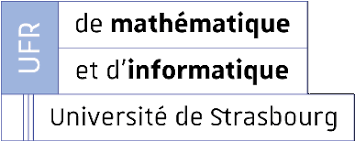
\includegraphics[scale=0.5]{images/logo_unistra.png}
        \end{figure}
        %{\large\bfseries \Autor}\\[1cm]
        {\large Date de rendu: \AbgabeDatum}\\[2cm]
        {\large Par}\\[0.5cm]
        {\large Matthieu FREITAG}\\[0.15cm]
        {\large et Paul MEYER}\\[3cm]
        {\large \href{https://github.com/Zapharaos/ProjetAI}{https://github.com/Zapharaos/ProjetAI}}
        \vfill
    \end{center}
\end{titlepage}
\clearpage

\pagestyle{plain}
%%%%%%%%%%%%%%%%%%%%%%%%%%%%%%%%%%%%%%%%%%%%%%%%%%%%%%%%%%%%%%%%%%%%%%%%%%%%%%%%%%%%

% Verzeichnisse
\setcounter{tocdepth}{1}

\renewcommand\contentsname{\usekomafont{chapter}\mdseries Index} % Ohne diese haben die überschriften der Verzeichnisse die komische komafont-schriftart
\tableofcontents

\printnoidxglossary[type=\acronymtype,title=Abréviations,toctitle=Abréviations] % Abkürzungen
\clearpage 
 
\setglossarystyle{altlist} % Danach Style auf "ausführlichere" Liste umschalten
\printnoidxglossary[nonumberlist] % Glossar, ohne Seitenzahlen für Referenzen
\clearpage

%\lstlistoflistings

%\renewcommand\listfigurename{\usekomafont{chapter}\mdseries Abbildungsverzeichnis}
%\listoffigures

%\renewcommand\listtablename{\usekomafont{chapter}\mdseries Tabellenverzeichnis}
%\listoftables

\clearpage

%\include{abk}

% -------------
%  Body Matter
% -------------

\pagenumbering{arabic}
\setcounter{page}{1}
\pagestyle{maincontentstyle}
 
%\include{einleitung}
\chapter{Introduction}

Dans ce projet, nous proposerons l'étude de différents modèles d'intelligence artificielle.

\section*{\color{black}Approche proposée}

Nous effectuerons cette étude grâce aux travaux pratiques effectués au préalable en python, et nous réaliserons les modèles suivants :
\begin{enumerate}
\item Arbres de décision
\item Réseau de neurones artificels
\end{enumerate}

Pour ce faire, nous débuterons par une préparation des données, après quoi nous pourrons procéder à la réalisation des différents modèles. Ensuite, nous analyserons ces modèles, puis les comparerons.

Note : Nous utiliserons les prédictions et les données de test fournies avec le sujet pour effetuer les parties d'analyse et de comparaison, mais nous en profiterons tout de même pour les comparer à notre implémentation.
\chapter{Préparation des données}

Ces données comportent quatorze attributs et les instances sont catégorisées en quatre classes différentes : \texttt{0}, \texttt{1}, \texttt{2}, \texttt{3}. Ces classes comptent respectivement \texttt{674}, \texttt{908}, \texttt{472}, et \texttt{244} instances.

D'après la figure \texttt{1} du sujet, les données ne sont pas linéairement séparables. En effet, on remarque un éparpillement des données et des regroupements entre classes qui rendent impossible la séparation des données. Par exemple : le point \texttt{(10, 11)} où les quatres classes sont présentes.

On distingue deux types de données : les données labelisées et les données numériques. Dans le cas d'un arbre de décision, il est possible d'utiliser des données labelisées, auquel cas il n'est alors pas nécessaire d'encoder en \texttt{one-hot}, ni de normaliser les données.

En revanche, avec un réseau de neurones, il est nécessaire d'utiliser des données numériques. Cependant, des données numériques simples ne sont pas suffisantes car le résultat risque d'être faussé à cause notamment d'un ordonnancement implicites des données, c'est pourquoi on a alors recours à un encodage en \texttt{one-hot}. Dans ce même contexte, il est utile de normaliser les données car, en plus d'améliorer les performances du modèle, cela permet d'équilibrer les données.

Séparer les données en un jeu d'entraînement et un jeu de test, permet tout d'abord de vérifier, via le jeu de test, que l'entraînement a correctement fonctionné. On utilise alors le taux d'erreur qui permet également de vérifier les erreurs, c'est-à-dire de s'assurer que le modèle n'est pas sous-entraîné ou sur-entraîné ce qui aménerait notamment à un modèle inadéquat.
\chapter{Mise en œuvre des modèles}

\section{Arbre de décision}

Nous n'avons malheureusement pas eu le temps d'effectuer cette partie.

\section{Réseaux de neurones artificiels}

Concernant cette partie, notre réseaux de neurones fonctionne, il nous manque uniquement l'implémentation de l'early-stopping. Cependant, nous allons tout de même procéder à une analyse détaillée de notre implémentation et la comparer aux résultats qui accompagnent le sujet afin de vérifier son bon fonctionnement.

Nous avons décidé d'aller plus loin en implémentant des fonctions d'initialisation de poids différentes (\texttt{xavier} et \texttt{he-et-al}). Afin de voir si l'une ou l'autre est plus intéressante à utiliser, nous avons entrainé chaque modèle une fois avec \texttt{xavier} et une autre avec \texttt{he-et-al}. Pour chaque entrainement nous avons généré les schémas de la matrice de confusion et des taux d'erreur.

Ne voulant pas surcharger, les données que nous analyserons ici ne seront pas intégrées dans ce rapport. En revanche, elles sont accessibles depuis l'archive dans \texttt{report/our-analysis}.

Pour les modèles \texttt{6-4}, on remarque que les résultats sont sensiblement similaires.
A partir des modèles \texttt{10-8-4}, on remarque que \texttt{xavier} a tendance à obtenir un nombre d'erreurs tout de même supérieur à son homologue \texttt{he-et-al}. En revanche, pour les modèles \texttt{10-8-6}, on remarque que \texttt{Relu he-et-al} performe moins bien, mais les résultats demeurent corrects.

La partie suivante est effectuée après les analyses de fin de rapport, ne voulant pas tout mélanger, nous en parlons donc ici.

De manière générale, on remarque que nos modèles \texttt{Relu} possèdent tout de même un nombre d'erreurs plus elevé que les résultats qui accompagnent le sujet. Cependant, l'inverse est facilement observable pour les modèles \texttt{Tanh}, excepté \texttt{10-8-6}. Cela ce remarque notamment grâce aux matrices de confusion.

Finalement, on remarque encore une fois que c'est le modèle \texttt{Tanh 10-8-6}, en particulier sa version \texttt{he-et-al}, qui obtient les meilleurs résultats, ce qui nous conforte dans notre analyse.

A titre d'information, voici la courbe des erreurs de ce modèle.

\begin{table}[H]
    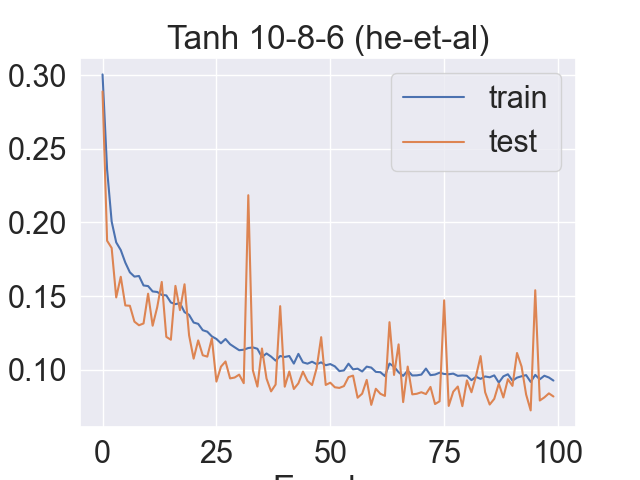
\includegraphics[scale=0.6]{images/tanh-10-8-6-errors.png}
    \caption{\label{HomePage} Schéma du taux d'erreurs en fonction de l'epoch (Tanh \texttt{10-8-6})}
\end{table}
\chapter{Analyse des modèles}

\begin{enumerate}
    \item Exactitude : le nombre de prédictions correctes sur le nombre de prédictions totales.
    \item Précision : le nombre de patients correctement identifiés comme malade sur le nombre de patients identifiés comme malade.
    \item Rappel : le nombre de patients correctement identifiés comme malade sur le nombre de patients malade.
    \item Score F1 : le rapport entre précision et rappel.
\end{enumerate}

\section{Modèle \texttt{DT4}}

\begin{table}[ht]
  \begin{tabular}{ m{5em} | m{1cm}| m{1cm} | m{1cm}| m{1cm} | } 
  \cline{2-5}
             & \multicolumn{4}{|c|}{Modèle \texttt{DT4}}\\
 \hline
 \multicolumn{1}{|c|}{\textit{Classes}} & \hfil \texttt{c1} & \hfil \texttt{c2} & \hfil \texttt{c3} & \hfil \texttt{c4} \\ 
  \hline
  \multicolumn{1}{|c|}{Accuracy} & \hfil 0.83 & \hfil 0.86 & \hfil 0.84 & \hfil 0.90 \\ 
  \hline
  \multicolumn{1}{|c|}{Precision} & \hfil 0.71 & \hfil 0.76 & \hfil 0.59 & \hfil 0.67 \\ 
  \hline
  \multicolumn{1}{|c|}{Recall} & \hfil 0.83 & \hfil 0.89 & \hfil 0.49 & \hfil 0.12 \\ 
  \hline
  \multicolumn{1}{|c|}{F1-score} & \hfil 0.77 & \hfil 0.82 & \hfil 0.54 & \hfil 0.21 \\ 
  \hline
\end{tabular}
\caption{Classification report pour le modèle \texttt{DT4}}
  \label{Tab:Tcr}
\end{table}

\begin{table}[H]
    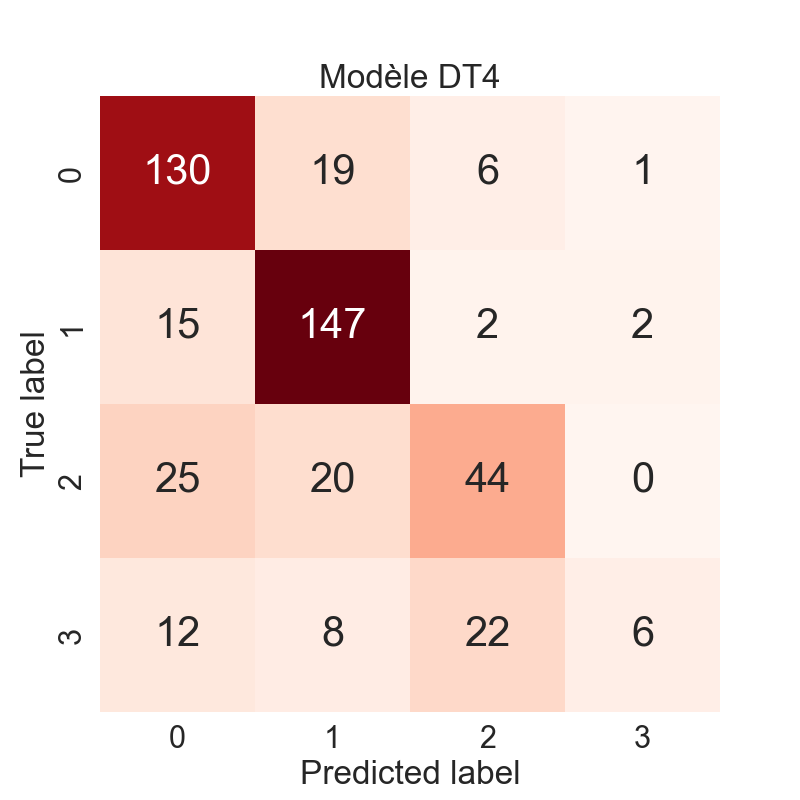
\includegraphics[scale=0.4]{images/y_pred_DT4.png}
    \caption{\label{HomePage} Matrice de confusion pour le modèle \texttt{DT4}}
\end{table}

\newpage

\section{Modèle \texttt{DT5}}

\begin{table}[ht]
  \begin{tabular}{ m{5em} | m{1cm}| m{1cm} | m{1cm}| m{1cm} | } 
  \cline{2-5}
             & \multicolumn{4}{|c|}{Modèle \texttt{DT5}}\\
 \hline
 \multicolumn{1}{|c|}{\textit{Classes}} & \hfil \texttt{c1} & \hfil \texttt{c2} & \hfil \texttt{c3} & \hfil \texttt{c4} \\ 
  \hline
  \multicolumn{1}{|c|}{Accuracy} & \hfil 0.87 & \hfil 0.89 & \hfil 0.88 & \hfil 0.91\\ 
  \hline
  \multicolumn{1}{|c|}{Precision} & \hfil 0.80 & \hfil 0.85 & \hfil 0.66 & \hfil 0.57 \\ 
  \hline
  \multicolumn{1}{|c|}{Recall} & \hfil 0.81 & \hfil 0.84 & \hfil 0.75 & \hfil 0.44 \\ 
  \hline
  \multicolumn{1}{|c|}{F1-score} & \hfil 0.81 & \hfil 0.85 & \hfil 0.71 & \hfil 0.49 \\ 
  \hline
\end{tabular}
\caption{Classification report pour le modèle \texttt{DT5}}
  \label{Tab:Tcr}
\end{table}

\begin{table}[H]
    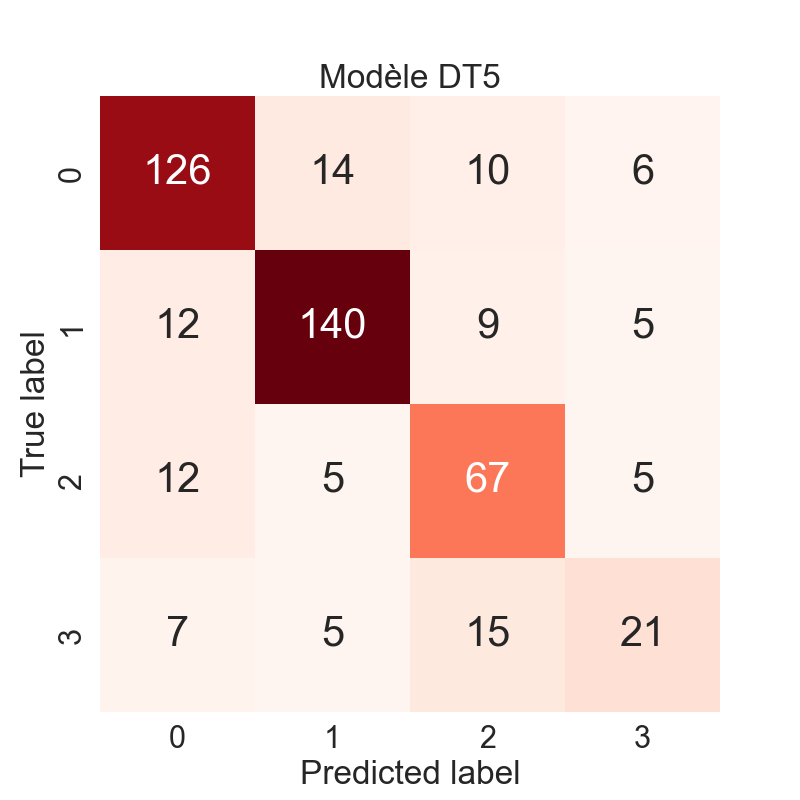
\includegraphics[scale=0.5]{images/y_pred_DT5.png}
    \caption{\label{HomePage} Matrice de confusion pour le modèle \texttt{DT5}}
\end{table}

\newpage

\section{Modèle \texttt{DT6}}

\begin{table}[ht]
  \begin{tabular}{ m{5em} | m{1cm}| m{1cm} | m{1cm}| m{1cm} | } 
  \cline{2-5}
             & \multicolumn{4}{|c|}{Modèle \texttt{DT6}}\\
 \hline
 \multicolumn{1}{|c|}{\textit{Classes}} & \hfil \texttt{c1} & \hfil \texttt{c2} & \hfil \texttt{c3} & \hfil \texttt{c4} \\ 
  \hline
  \multicolumn{1}{|c|}{Accuracy} & \hfil 0.89 & \hfil 0.90 & \hfil 0.91 & \hfil 0.93 \\ 
  \hline
  \multicolumn{1}{|c|}{Precision} & \hfil 0.85 & \hfil 0.84 & \hfil 0.75 & \hfil 0.69 \\ 
  \hline
  \multicolumn{1}{|c|}{Recall} & \hfil 0.83 & \hfil 0.89 & \hfil 0.80 & \hfil 0.52 \\ 
  \hline
  \multicolumn{1}{|c|}{F1-score} & \hfil 0.84 & \hfil 0.86 & \hfil 0.77 & \hfil 0.60 \\ 
  \hline
\end{tabular}
\caption{Classification report pour le modèle \texttt{DT6}}
  \label{Tab:Tcr}
\end{table}

\begin{table}[H]
    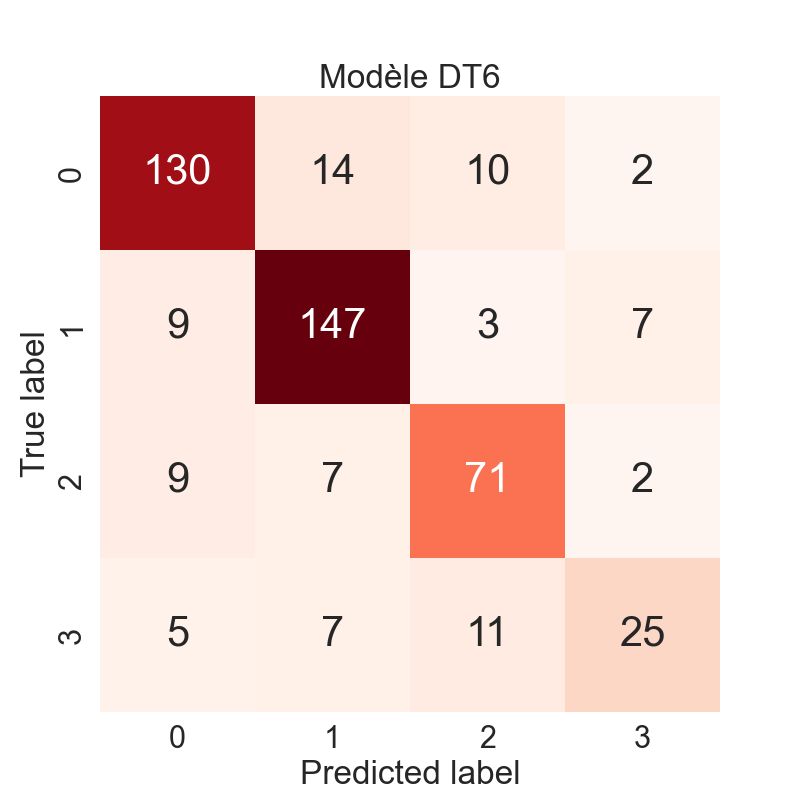
\includegraphics[scale=0.5]{images/y_pred_DT6.png}
    \caption{\label{HomePage} Matrice de confusion pour le modèle \texttt{DT6}}
\end{table}

\newpage

\section{Modèle \texttt{NN relu 6-4}}

\begin{table}[ht]
  \begin{tabular}{ m{5em} | m{1cm}| m{1cm} | m{1cm}| m{1cm} | } 
  \cline{2-5}
             & \multicolumn{4}{|c|}{Modèle \texttt{NN relu 6-4}}\\
 \hline
 \multicolumn{1}{|c|}{\textit{Classes}} & \hfil \texttt{c1} & \hfil \texttt{c2} & \hfil \texttt{c3} & \hfil \texttt{c4} \\ 
  \hline
  \multicolumn{1}{|c|}{Accuracy} & \hfil 0.94 & \hfil 0.95 & \hfil 0.94 & \hfil 0.92 \\ 
  \hline
  \multicolumn{1}{|c|}{Precision} & \hfil 0.94 & \hfil 0.91 & \hfil 0.79 & \hfil 0.65 \\ 
  \hline
  \multicolumn{1}{|c|}{Recall} & \hfil 0.87 & \hfil 0.95 & \hfil 0.92 & \hfil 0.50 \\ 
  \hline
  \multicolumn{1}{|c|}{F1-score} & \hfil 0.90 & \hfil 0.93 & \hfil 0.85 & \hfil 0.56 \\ 
  \hline
\end{tabular}
\caption{Classification report pour le modèle \texttt{NN relu 6-4}}
  \label{Tab:Tcr}
\end{table}

\begin{table}[H]
    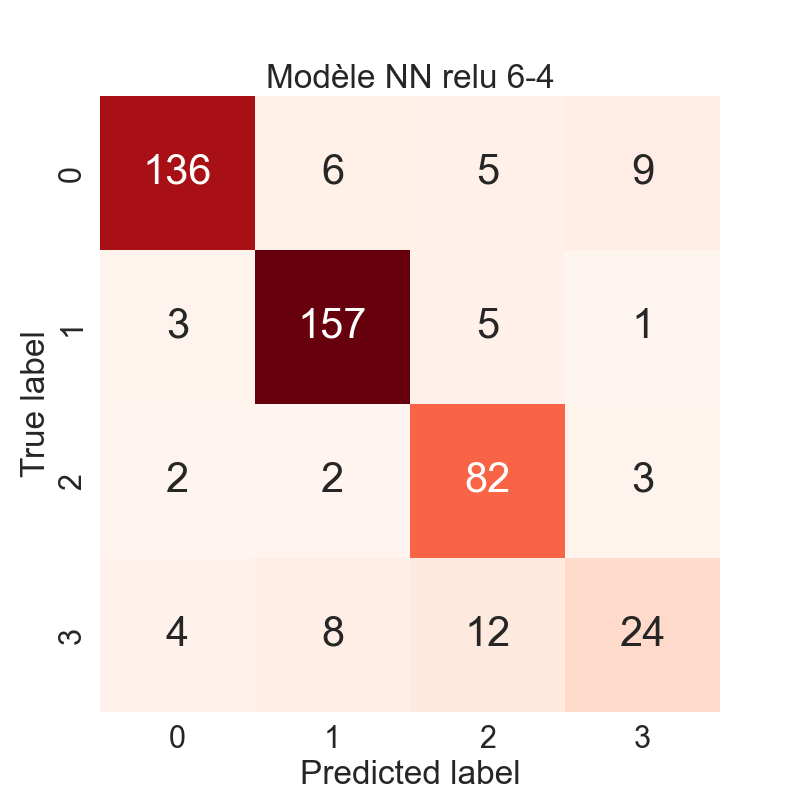
\includegraphics[scale=0.5]{images/y_pred_NN_relu_6-4.png}
    \caption{\label{HomePage} Matrice de confusion pour le modèle \texttt{NN relu 6-4}}
\end{table}

\newpage

\section{Modèle \texttt{NN relu 10-8-4}}

\begin{table}[ht]
  \begin{tabular}{ m{5em} | m{1cm}| m{1cm} | m{1cm}| m{1cm} | } 
  \cline{2-5}
             & \multicolumn{4}{|c|}{Modèle \texttt{NN relu 10-8-4}}\\
 \hline
 \multicolumn{1}{|c|}{\textit{Classes}} & \hfil \texttt{c1} & \hfil \texttt{c2} & \hfil \texttt{c3} & \hfil \texttt{c4} \\ 
  \hline
  \multicolumn{1}{|c|}{Accuracy} & \hfil 0.95 & \hfil 0.94 & \hfil 0.95 & \hfil 0.93 \\ 
  \hline
  \multicolumn{1}{|c|}{Precision} & \hfil 0.97 & \hfil 0.87 & \hfil 0.84 & \hfil 0.71 \\ 
  \hline
  \multicolumn{1}{|c|}{Recall} & \hfil 0.87 & \hfil 0.98 & \hfil 0.91 & \hfil 0.52 \\ 
  \hline
  \multicolumn{1}{|c|}{F1-score} & \hfil 0.92 & \hfil 0.92 & \hfil 0.87 & \hfil 0.60 \\ 
  \hline
\end{tabular}
\caption{Classification report pour le modèle \texttt{NN relu 10-8-4}}
  \label{Tab:Tcr}
\end{table}

\begin{table}[H]
    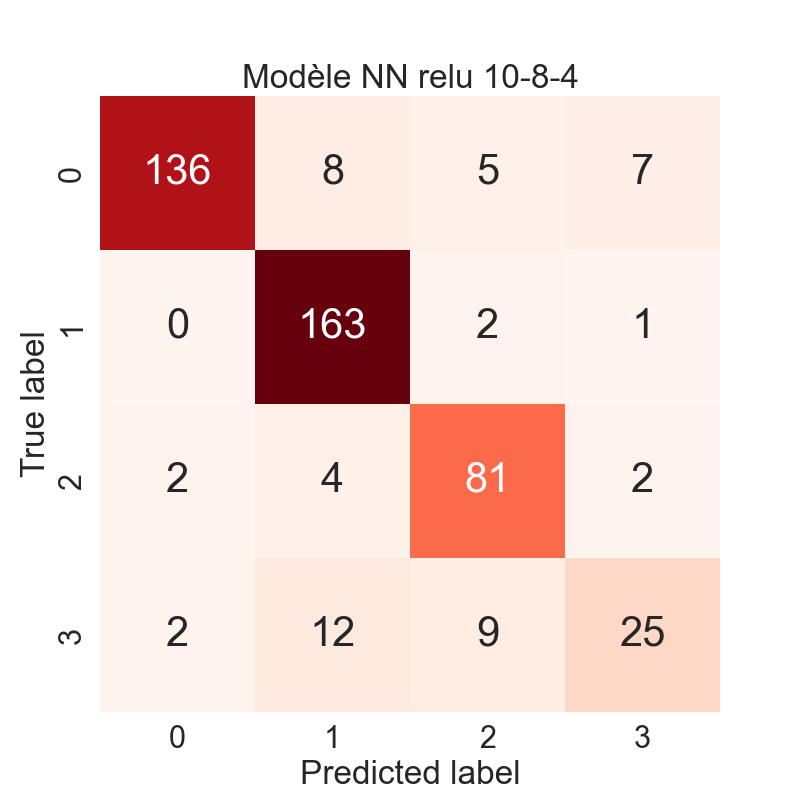
\includegraphics[scale=0.5]{images/y_pred_NN_relu_10-8-4.png}
    \caption{\label{HomePage} Matrice de confusion pour le modèle \texttt{NN relu 10-8-4}}
\end{table}

\newpage

\section{Modèle \texttt{NN relu 10-8-6}}

\begin{table}[ht]
  \begin{tabular}{ m{5em} | m{1cm}| m{1cm} | m{1cm}| m{1cm} | } 
  \cline{2-5}
             & \multicolumn{4}{|c|}{Modèle \texttt{NN relu 10-8-6}}\\
 \hline
 \multicolumn{1}{|c|}{\textit{Classes}} & \hfil \texttt{c1} & \hfil \texttt{c2} & \hfil \texttt{c3} & \hfil \texttt{c4} \\ 
  \hline
  \multicolumn{1}{|c|}{Accuracy} & \hfil 0.95 & \hfil 0.94 & \hfil 0.94 & \hfil 0.92 \\ 
  \hline
  \multicolumn{1}{|c|}{Precision} & \hfil 0.97 & \hfil 0.90 & \hfil 0.81 & \hfil 0.63 \\ 
  \hline
  \multicolumn{1}{|c|}{Recall} & \hfil 0.87 & \hfil 0.93 & \hfil 0.90 & \hfil 0.65 \\ 
  \hline
  \multicolumn{1}{|c|}{F1-score} & \hfil 0.92 & \hfil 0.92 & \hfil 0.85 & \hfil 0.64 \\ 
  \hline
\end{tabular}
\caption{Classification report pour le modèle \texttt{NN relu 10-8-6}}
  \label{Tab:Tcr}
\end{table}

\begin{table}[H]
    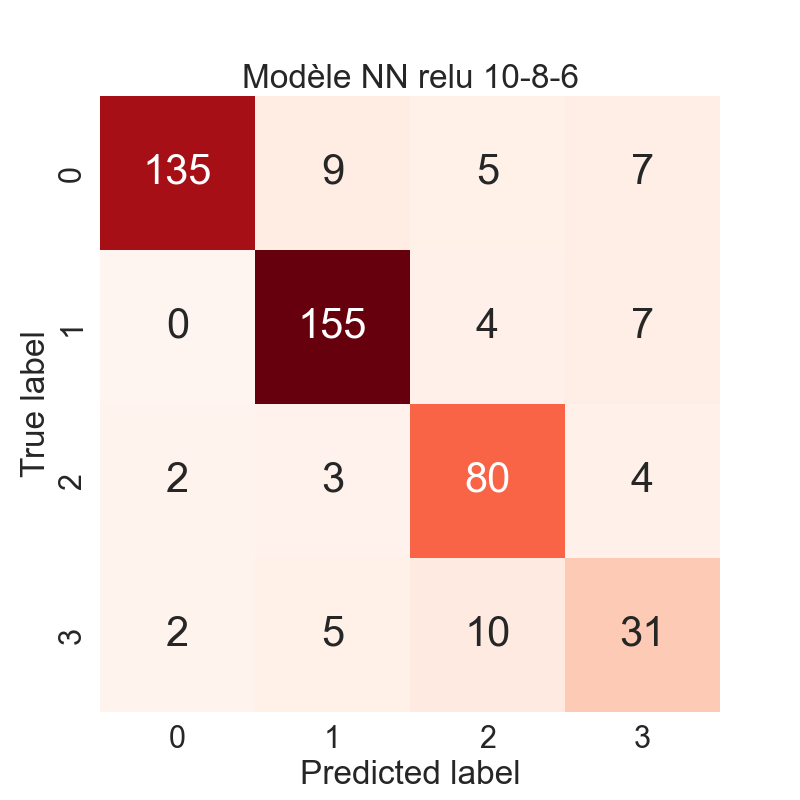
\includegraphics[scale=0.5]{images/y_pred_NN_relu_10-8-6.png}
    \caption{\label{HomePage} Matrice de confusion pour le modèle \texttt{NN relu 10-8-6}}
\end{table}

\newpage

\section{Modèle \texttt{NN tanh 6-4}}

\begin{table}[ht]
  \begin{tabular}{ m{5em} | m{1cm}| m{1cm} | m{1cm}| m{1cm} | } 
  \cline{2-5}
             & \multicolumn{4}{|c|}{Modèle \texttt{NN tanh 6-4}}\\
 \hline
 \multicolumn{1}{|c|}{\textit{Classes}} & \hfil \texttt{c1} & \hfil \texttt{c2} & \hfil \texttt{c3} & \hfil \texttt{c4} \\ 
  \hline
  \multicolumn{1}{|c|}{Accuracy} & \hfil 0.91 & \hfil 0.94 & \hfil 0.92 & \hfil 0.90 \\ 
  \hline
  \multicolumn{1}{|c|}{Precision} & \hfil 0.85 & \hfil 0.87 & \hfil 0.75 & \hfil 0.00 \\ 
  \hline
  \multicolumn{1}{|c|}{Recall} & \hfil 0.89 & \hfil 0.99 & \hfil 0.89 & \hfil 0.00 \\ 
  \hline
  \multicolumn{1}{|c|}{F1-score} & \hfil 0.87 & \hfil 0.93 & \hfil 0.81 & \hfil 0.00 \\ 
  \hline
\end{tabular}
\caption{Classification report pour le modèle \texttt{NN tanh 6-4}}
  \label{Tab:Tcr}
\end{table}

\begin{table}[H]
    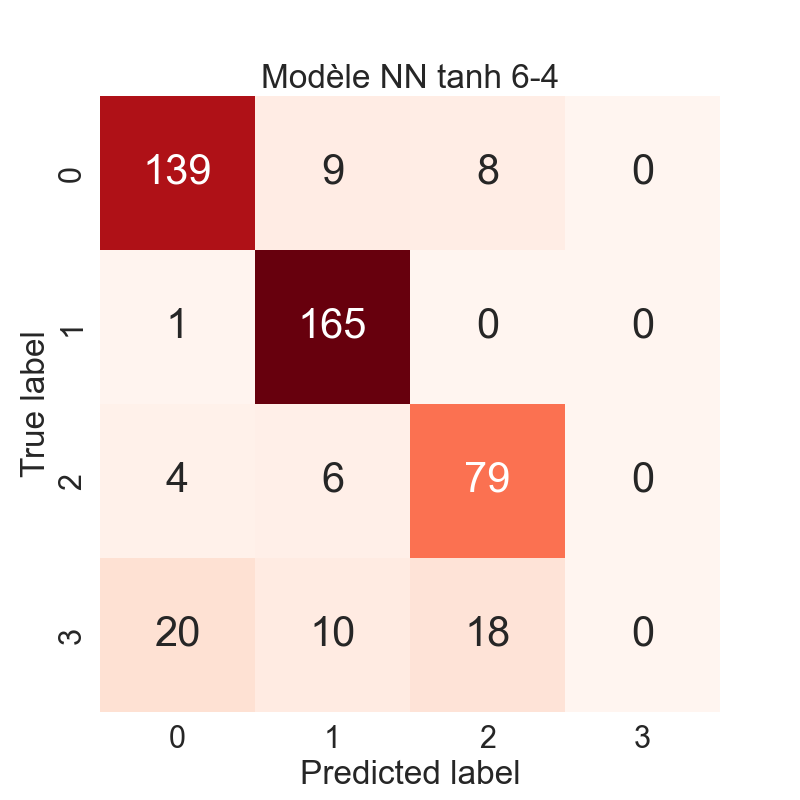
\includegraphics[scale=0.5]{images/y_pred_NN_tanh_6-4.png}
    \caption{\label{HomePage} Matrice de confusion pour le modèle \texttt{NN tanh 6-4}}
\end{table}

\newpage

\section{Modèle \texttt{NN tanh 10-8-4}}

\begin{table}[ht]
  \begin{tabular}{ m{5em} | m{1cm}| m{1cm} | m{1cm}| m{1cm} | } 
  \cline{2-5}
             & \multicolumn{4}{|c|}{Modèle \texttt{NN tanh 10-8-4}}\\
 \hline
 \multicolumn{1}{|c|}{\textit{Classes}} & \hfil \texttt{c1} & \hfil \texttt{c2} & \hfil \texttt{c3} & \hfil \texttt{c4} \\ 
  \hline
  \multicolumn{1}{|c|}{Accuracy} & \hfil 0.94 & \hfil 0.94 & \hfil 0.92 & \hfil 0.90 \\ 
  \hline
  \multicolumn{1}{|c|}{Precision} & \hfil 0.90 & \hfil 0.87 & \hfil 0.74 & \hfil 0.00 \\ 
  \hline
  \multicolumn{1}{|c|}{Recall} & \hfil 0.91 & \hfil 0.98 & \hfil 0.94 & \hfil 0.00 \\ 
  \hline
  \multicolumn{1}{|c|}{F1-score} & \hfil 0.91 & \hfil 0.92 & \hfil 0.83 & \hfil 0.00 \\ 
  \hline
\end{tabular}
\caption{Classification report pour le modèle \texttt{NN tanh 10-8-4}}
  \label{Tab:Tcr}
\end{table}

\begin{table}[H]
    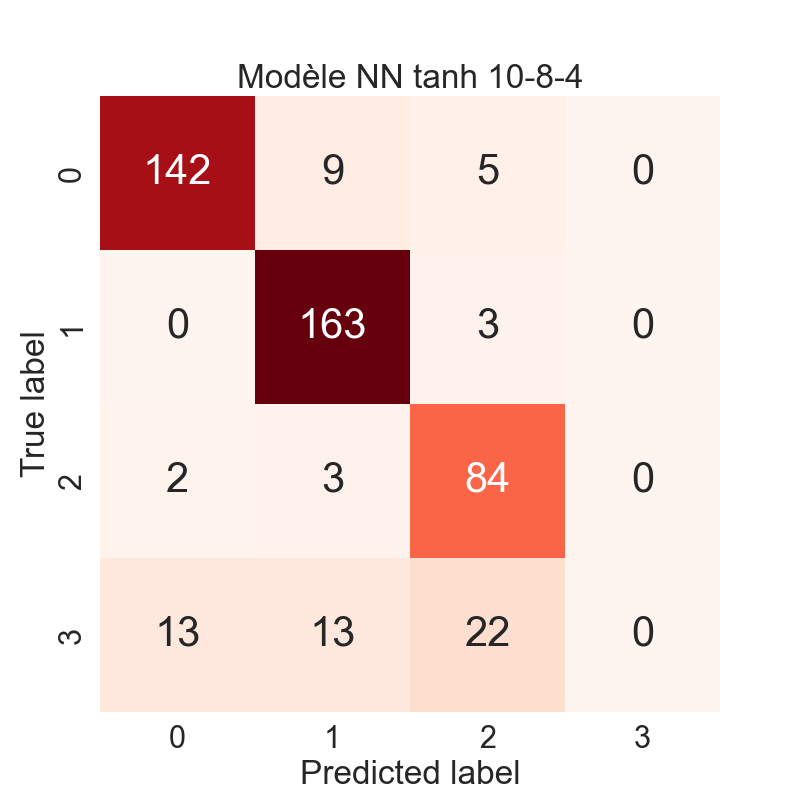
\includegraphics[scale=0.5]{images/y_pred_NN_tanh_10-8-4.png}
    \caption{\label{HomePage} Matrice de confusion pour le modèle \texttt{NN tanh 10-8-4}}
\end{table}

\newpage

\section{Modèle \texttt{NN tanh 10-8-6}}

\begin{table}[ht]
  \begin{tabular}{ m{5em} | m{1cm}| m{1cm} | m{1cm}| m{1cm} | } 
  \cline{2-5}
             & \multicolumn{4}{|c|}{Modèle \texttt{NN tanh 10-8-6}}\\
 \hline
 \multicolumn{1}{|c|}{\textit{Classes}} & \hfil \texttt{c1} & \hfil \texttt{c2} & \hfil \texttt{c3} & \hfil \texttt{c4} \\ 
  \hline
  \multicolumn{1}{|c|}{Accuracy} & \hfil 0.96 & \hfil 0.95 & \hfil 0.97 & \hfil 0.94 \\ 
  \hline
  \multicolumn{1}{|c|}{Precision} & \hfil 0.97 & \hfil 0.90 & \hfil 0.91 & \hfil 0.78 \\ 
  \hline
  \multicolumn{1}{|c|}{Recall} & \hfil 0.92 & \hfil 0.98 & \hfil 0.91 & \hfil 0.65 \\ 
  \hline
  \multicolumn{1}{|c|}{F1-score} & \hfil 0.94 & \hfil 0.93 & \hfil 0.91 & \hfil 0.70 \\ 
  \hline
\end{tabular}
\caption{Classification report pour le modèle \texttt{NN tanh 10-8-6}}
  \label{Tab:Tcr}
\end{table}

\begin{table}[H]
    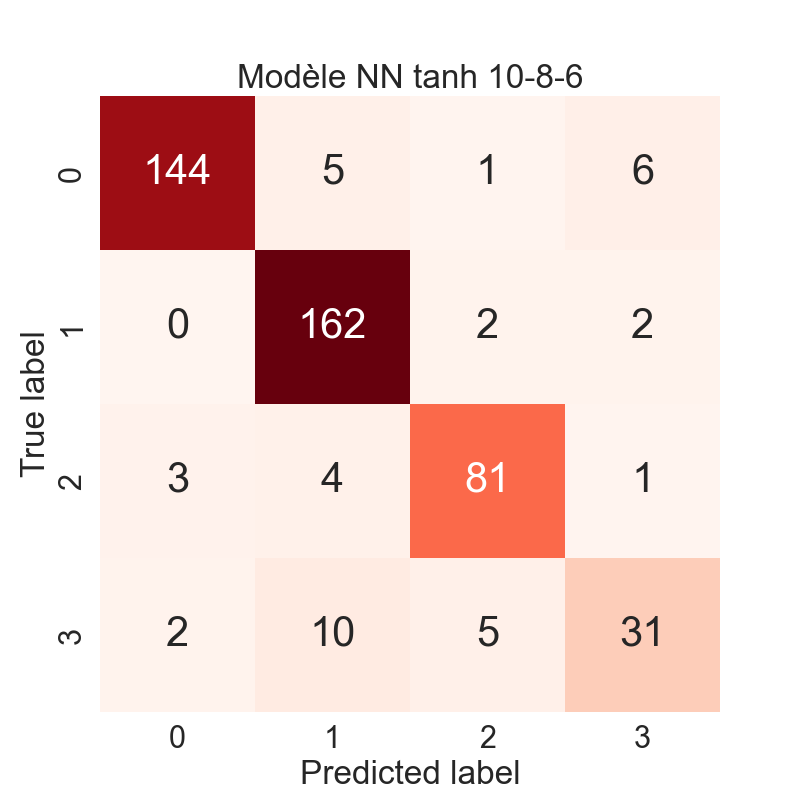
\includegraphics[scale=0.5]{images/y_pred_NN_tanh_10-8-6.png}
    \caption{\label{HomePage} Matrice de confusion pour le modèle \texttt{NN tanh 10-8-6}}
\end{table}

\newpage
\chapter{Le meilleure modèle}

\section{Comparaison des modèles}

On rappelle d'abord que les classes \texttt{2} et \texttt{3} possèdent des instances plus faible que les classes \texttt{0} et \texttt{1}, ce qui explique notamment pourquoi elles peuvent posséder certaines métriques abérrantes par moment.

On remarque aisément, via les classification reports, que les arbres de décision possèdent une exactitude et une précision qui augmente graduellement avec la profondeur, tandis que le rappel et le score F1 ont plutôt tendance à être stable. \newline
Ensuite, concernant les réseaux neuronaux, on remarque que les métriques conservent, peu importe la profondeur, une certaine stabilité.

Notre analyse précédente sur les classification reports se confirment ici. On retrouve, dans nos matrices de confusion, notre croissance pour les arbres de décisions et notre stabilité pour les réseaux neuronaux. On remarque également un nombre d'erreurs plus important pour les classes \texttt{2} et \texttt{3}, et en particulier la classe \texttt{3}.

Ainsi, le modèle "NN tanh 10-8-6" nous apparaît évidemment comme étant le meilleur modèle. En effet, il est celui qui possède les meilleures métriques. L'exactitude élevée montre que la majorité des prédictions se sont avérées être correctes. La précision et le rappel du modèle le confirment : le modèle possède un faible taux d'erreur (i.e. une précision et un rappel élevé). Autrement dit, peu de patients (malade ou sains) ont été incorrectement diagnostiqué. De plus, le fait que le score F1 soit élevé montre que le rapport précision/rappel est optimal.

\newpage

\section{Les types de modèles}

On remarque effectivement que les différences entre les arbres de décision et les réseaux de neurones ne sont pas très grandes. Pourtant, de manière générale et d'après nos analyses, ce sont les réseaux neuronaux qui se démarquent le plus. En effet, ces derniers possèdent une exactitude bien supérieure à celle des arbres binaires et le score F1 indique un meilleur rapport précision/rappel. Ceci signifie notamment que le taux d'erreur est plus faible pour les réseaux de neurones et que, par conséquent, ils ont plus fiables. Ceci est un point particulièrement important dans le cadre de diagnostiques médicaux.

Cependant, les réseaux neuronaux sont extrêmement complexes. A tel point que cela complique la justification des décisions prises par ce modèle. Cela découle naturellement du nombre de calculs et de noeuds que réalise ce modèle, tandis que les arbres de décisions sont beaucoup plus simples. En effet, rien que d'un point de vu graphique, les justifications sont plus compréhensible. C'est pourquoi, si nous devions justifier un diagnostic médical, nous aurions alors tendance à privilégier les arbres de décision aux réseaux de neurones.
\chapter{Conclusion}

Dans l'objectif d'une amélioration future, il serait d'abord nécessaire de terminer l'implémentation demandée. En plus de l'early-stopping pour les réseaux de neurones, la partie sur les arbres de décisions est manquante. Nous avons rencontré un grand nombre de problèmes lors de la réalisation des réseaux de neurones et, par conséquent, avons perdu beaucoup de temps.

Il serait également intéressant de réaliser ce projet avec des bibliothèques comme \texttt{TensorFlow}.

%\include{deployment}
%\chapter{Anhang}
%\includepdf[pages=1]{LogFiles.pdf}

\clearpage

% -------------
%  Back Matter
% -------------

{
    \setstretch{1.1}
    \renewcommand{\bibfont}{\normalfont\small}
    \setlength{\bibitemsep}{0.5\baselineskip plus 0.5\baselineskip}
    \emergencystretch=1em
    \printbibliography 
}
\end{document}